% =========================================================================
% 《高中數學實驗教材》第二冊（高一下） 
% 第五章 對數表的用法與計算尺原理*
% =========================================================================

\section{對數表的用法與計算尺原理\texorpdfstring{$^*$}{*}}\label{sec:b2_ch5}

\subsection{對數表}

在算術四則的計算裏，加減比乘除要簡單多了——尤其是有一堆很大的數目字的時候，更是如此.（不信，你就計算 $3.2705319 \times 927.6412195$ 和 $3.2705319 + 927.6412195$ 比較看看！）即使我們只想得到一個近似值，乘除也會比加減麻煩得多.

對數函數的發明和對數函數表的利用，就是使我們能夠將乘除的計算改成加減的，並且使它器械化！

假設 $a$ 是一個不等於 1 的正數，而且用 $a$ 做底的對數函數已經編列成表，也就是說對任一個正數 $x$，$\log_a x$ 一查便知，而它的反函數卽指數函數 $a^x$，也一查便知. 那麼要知道兩個正數 $x, y$ 的乘積 $xy$，只需先知道 $\log_a xy$，剩下就只要查表了.（動眼睛不動手！）

但因為
\[
\log_a xy = \log_a x + \log_a y,
\]
我們只需先查出 $\log_a x$ 和 $\log_a y$，做加法運算（只有在這裏要動手！），就得到 $\log_a xy$ 了！\footnote{計算尺之使用不在部頒課程標準之內，但其原理極其簡單，爲對數計算之一應用而已，並且在實際計算時使用計算尺極為方便，高中同學皆應了解計算尺原理及簡單使用方法，並可在物理學、化學課程中使用。如因教學時間限制，亦可略去不講，留供同學自行參考。}

同樣的道理要計算 $z = \frac{xy}{uvw}$（設 $x, y, u, v, w$ 都是正數），我們可以這麼做：
\begin{enumerate}[(1)]
    \item 查表得出 $\log_a x, \log_a y, \log_a u, \log_a v, \log_a w$.
    \item 算出 $S = \log_a x + \log_a y - \log_a u - \log_a v - \log_a w$.
    \item 查表找出正數 $z$ 使得 $\log_a z = S$.
\end{enumerate}

\paragraph{【例 1】} 求
\[
\frac{3.67 \times 4.92 \times 7.25}{9.75 \times 8.73}
\]

\paragraph{【解】}
\begin{align*}
\text{查表得} \qquad \log_{10} 3.67 &= 0.5647 & \log_{10} 9.75 &= 0.9890 \\
\log_{10} 4.92 &= 0.6920 & +\;)\; \log_{10} 8.73 &= 0.9405 \\
\cline{4-4}
+\;)\; \log_{10} 7.25 &= 0.8603 & & 1.9295 \\
\cline{2-2}
& 2.1170
\end{align*}
\[
2.1170 - 1.9295 = 0.1875.
\]
\[
\log_{10} 1.54 = 0.1875. \qquad \therefore \text{答案是 } 1.54.
\]

通常用的對數表只有兩種，一種是用 10 做底數的，叫做「常用」對數表. 一種是用一個特別重要的數 $e = 2.71828\dots\dots$ 作底數的，叫做「自然」對數表，後者特別在高等數學裏有極重要的理論價值，但是我們現在只對常用對數有興趣，因此以下就用 $\log$ 代替 $\log_{10}$.

為什麼 10 是最實用的對數呢？這是因爲人類用慣了十進位制的原故. 由公式 $\log xy = \log x + \log y$，我們的對數表只需列上區間 $1 < x < 10$ 裏的 $x$ 的對數，譬如說
\begin{align*}
\log 497 &= \log(100 \times 4.97) \\
&= \log 100 + \log 4.97 = 2 + 0.6964 \\
&= 2.6964.
\end{align*}
而 $\log 0.0000497 = -5 + 0.6964 = -4.3036$.

在對數表所列的對數值幾乎全是近似值，因此我們在計算時一定得有近似值計算法的常識. 我們特別提到下面兩點：

\subsubsection{精確度}

每個正數 $a$ 都可以化成一個 10 的倍數與個位數的乘積. 卽存在整數 $k$ 使得 $1 \le \frac{a}{10^k} < 10$，所以
\[
a = \left(\frac{a}{10^k}\right) 10^k.
\]
這叫做標準寫法（或科學記法）.

若取 $a$ 的對數，就得到 $k = [\log a]$，卽 $\log a$ 的整數部分. 另一方面，我們說 $\frac{a}{10^k}$ 是 $a$ 的有效數字部分，它的長度，亦卽 $\frac{a}{10^k}$ 的小數點下位數加 1，就叫 $a$ 的有效數字位數.

例如 $0.0000437$ 的有效數字是 $4.37$，有三位有效數字，而 $\log 0.0000437$ 的整數部分爲 $-5$，所以 $0.0000437$ 的標準寫法是
\[
4.37 \times 10^{-5}.
\]

在計算近似值時，我們必須指明精確到幾位有效數字. 例如 $0.09235716$ 若取三位有效數字的精確度，我們就寫成：
\[
9.24 \times 10^{-2}
\]
若是 $70,454,620,000$ 取四位有效數字的精確度就寫成
\[
7.045 \times 10^{10}.
\]

\paragraph{注意：} 前面例子有效數字中，最後一位數字都已經過四捨五入的處理了，如果最後一例中，取二位數字的精確度就要寫作
\[
7.0 \times 10^{10},
\]
不可以寫作 $7 \times 10^{10}$！

在一長串的乘除中，所得結果的精確度的位數不會大過各乘除因子精確度位數的最小者。這是我們最須緊記的一點！很多人最常患的錯誤是對一串乘積中的某一個因子苛刻地求其精確度，（例如精確到八，九位有效數字），而沒有考慮到當別的因子精確度太差時（例如只精確到三，四位），這種苛求就完全失去意義了.

\paragraph{【例 2】} $4.128 \times 2.953 = 12.189$\phantomsection\label{note:b2-ch5-p114-ex2}

\subsection*{習題 5-1}
\begin{enumerate}
    \item 某棟樓八十幾萬元，某乙說某物一斤值幾十元，兩個人誰比較沒有科學觀念？
    \item 已知 $47^{100}$ 爲 168 位數；試問 $47^{17}$ 爲幾位數？
    \item 氫原子的質量是 $0.000,000,000,000,000,000,000,001,6734\text{g}$（克），如何寫成標準形式.
    \item 求下列各對數：
    \begin{enumerate}[(i)]
        \item $\log \frac{1}{3.5 \times 2.64}$,
        \item $\log \frac{5070000}{2}$,
        \item $\log \frac{8.59 \times 9.75}{4.15}$,
    \end{enumerate}
    \item 利用對數算出下列各數的近似值至二位小數
    \begin{enumerate}[(i)]
        \item $\frac{3.99 \times 3.69}{4}$,
        \item $1530000 \times 0.0086$,
        \item $0.00251 \times 0.000379$,
    \end{enumerate}
\end{enumerate}

從實用的立場來說，對數表給出四位小數就已夠用了！另一個和表的精確度密切相關的觀念是表的細密度，像我們書後附錄的對數表就細密到三位有效數字，因爲對數表不可能把每個 1 到 10 之間的 $x$（$1 \le x < 10$）的對數 $\log x$ 都列出，例如表上沒有 $\log 7.4142$，只有 $\log 7.41, \log 7.42, \log 7.43$ 等等. 所以要計算 $\log 7.4142$ 就要用內插法.

\subsubsection{內插法查表}

就拿 $\log 7.4142$ 來討論：

\begin{center}
\renewcommand{\arraystretch}{1.2}
\begin{tabular}{c|c}
$x$ & $y = \log x$ \\ \hline
$7.42$ & $0.8704$ \\
$7.41$ & $0.8698$ \\ \hline
\text{差 } $\Delta x = 0.01$ & $\Delta y = 0.0006$
\end{tabular}
\end{center}

這 0.0006 是相當於 $x$ 自 7.41 變到 7.42 時 $y = \log x$ 的變化.

我們自然想問：如果 $x$ 自 7.41 變到 7.4142，$y$ 會變爲多少？

內插法的原理是：在一個很小的範圍內來說，$x$ 的微差和 $y$ 的微差近似地成比例. 在此來說，就是對 $y = \log 7.4142$，我們可以有：\phantomsection\label{note:b2-ch5-p115-interpolation-zero}
\begin{align*}
(y - 0.8698) : (7.4142 - 7.41) &= (0.8704 - 0.8698) : (7.42 - 7.41) \\
&= 0.0006 : 0.01 \\
y &= 0.8698 + 0.006 \cdot \frac{0.0042}{0.01} \\
&= 0.8698 + 0.000252 \\
&= 0.8701. \qquad\quad \text{答 } \log 7.4142 = 0.8701.
\end{align*}

讓我們再註解一下：0.0042 中的 2 不值得考慮，因爲這種精度不太有意義，所以如果答案寫作 0.8700 也未嘗不可，最後一位的誤差，完全在意料之中.

同學們請注意，比例內插法的校正數值表，通常就附在對數表內. 例如求 $\log 7.418$，查對數表得
\[
\log 7.41 = 0.8698
\]
$\Delta x = 7.418 - 7.41 = 0.008$，查所附校正數值表（對數表中最後三欄）讀出校正數值 $\Delta y = 0.0005$，所以
\[
\log 7.418 = 0.8698 + 0.0005 = 0.8703.
\]

\subsection*{習題 5-2}
\begin{enumerate}
    \item 比例內插法在圖解法上有什麼意義？
    \item 求下列對數：
    \begin{enumerate}[(i)]
        \item $\log 1024$,
        \item $\log 1547000$,
        \item $\log 0.000007698$,
        \item $\log 98690$,
        \item $\log 0.085741$.
    \end{enumerate}
\end{enumerate}

對數表 $\log x$ 中的 $x$ 都在 1 與 10 之間，因此 $\log x$ 都是介於 0 和 1 間的小數，而一般個位數以上的情形如：
\[
\log 7.41 = 0.8698, \; \log 74.1 = 1.8698 \text{ 及 } \log 7410 = 3.8698, \text{ 等等.}
\]
因此，爲一致且方便起見，對於小數的對數計算，都把 $\log 0.00741 = -3 + 0.8698$，記作 $\bar{3}.8698$；如果你眞去算出 $\log 0.00741 = -2.1302$，那常會是畫蛇添足，因為取對數值多半只是運算中的過程而不是目的.

\paragraph{【例 3】} $8.85 \times 0.762 \div 0.04796 = ?$

\paragraph{【解】}\phantomsection\label{note:b2-ch5-p116-ex3-minus-log}
\begin{align*}
\log 8.85 &= 0.9469, \\
\log 0.762 &= \bar{1}.8820 \\
-\quad \log 0.04796 &= 1.3192 \\
\cline{1-2}
\log ? &= 2.1481.
\end{align*}
\[
(\log 0.04796 = \bar{2}.6808)
\]
查表知 $\log 1.40 = 0.1461$.
\[
\Delta x \sim 0.007, \quad \Delta y = 21
\]
\[
\therefore \text{答案是 } 140.7.
\]

\paragraph{【例 4】} 求 $x = \sqrt[5]{0.00626}$

\paragraph{【解】}
\[
\log x = \frac{1}{5} \log 0.00626 = \frac{1}{5} (\bar{3}.7966)
\]
\[
= -0.6 + 0.15932 = \bar{1}.5593
\]
查表知
\[
\log 0.362 = \bar{1}.5587
\]
\[
\Delta y = 5593 - 5587 = 6,
\]
查校正數值表得
\[
\Delta x = 0.0005.
\]
\[
\text{答 } x = 0.3625.
\]

\paragraph{【例 5】} $u = \frac{4}{3} \pi \times 0.875^3$

\paragraph{【解】}
\begin{align*}
\log \pi &= 0.4971 & \log 3 &= 0.4771 \\
\log 4 &= 0.6021 & \log 0.875 &= \bar{1}.9420 \\
+\qquad & \bar{1}.3489 & \log 0.875^3 &= \bar{1}.8260 \\
\cline{1-2}
\log u &= 0.4481 & -0.4771 \\
\cline{3-4}
\log 2.80 &= 0.4472 & & \bar{1}.3489
\end{align*}
\[
\Delta y = 4481 - 4472 = 9,
\]
查出 $\Delta u = 0.006$
\[
\text{答 } u = 2.806.
\]

\subsection*{習題 5-3}
\begin{enumerate}
    \item 下列各數是那些數的對數？
    \begin{enumerate}[(i)]
        \item $2.7157$,
        \item $\bar{2}.7157$,
        \item $-2.7157$,
        \item $0.6990 + \bar{1}.5445 - 2.3098$,
        \item $\bar{1}.7082 + \bar{2}.4771 - \bar{3}.6021$.
    \end{enumerate}
    \item 求 $\sqrt[3]{0.5495}$.
    \item 求 $5.42 \times 3.5 \times 2.55 \div 8.12$.
    \item 求 $(9.29 \times 10^3)^5$.
    \item 利用對數求 $2^{10}$.
    \item 求正整數 $n$ 使 $4000 < (\frac{5}{4})^n < 5000$，利用 $\log_{10} 2 = 0.3010$.
    \item 已知 $\log 3 \fallingdotseq 0.4771$. 問 $(\frac{1}{3})^{20}$ 表成小數時，不等於 0 的第 1 個數字出現在那裏？
    \item 
    \begin{enumerate}[(i)]
        \item 求最小整數指數 $x$，使 $(\frac{4}{5})^x < 0.000001$；
        \item 求最小整數指數 $x$，使 $(\frac{3}{5})^x < 0.0001$.
    \end{enumerate}
    \item 
    \begin{enumerate}[(i)]
        \item 求最小整數指數 $x$，使 $(\frac{10}{9})^x > 1000000$；
        \item 求最小整數指數 $x$，使 $(\frac{9}{8})^x > 10000000$.
    \end{enumerate}
\end{enumerate}

\subsection{計算尺原理\texorpdfstring{$^*$}{*}}

上面已經說明如何利用對數和對數表把乘除化爲加減，也把乘方化爲倍數的（近似值）計算法. 這個辦法更可以和圖表或者器械配合起來使用，其中最重要最具實用價值的就是計算尺.\footnote{見 111 頁之說明.}

式子 $\log xy = \log x + \log y$，在器械上很容易表達出來：

\begin{center}
\begin{tikzpicture}[scale=1.0, line cap=round, line join=round]
    % --- Figure 1 (Left) ---
    \begin{scope}[shift={(0, 0)}]
        \draw[thick, |-|] (0, 1.3) -- (2.6, 1.3) node[midway, above=1pt] {\small $\log x$};
        \draw[thick, |-|] (2.6, 0.65) -- (3.9, 0.65) node[midway, above=1pt] {\small $\log y$};
        \draw[thick, |-|] (0, 0) -- (3.9, 0) node[midway, above=1pt] {\small $\log xy$};
        \node at (1.95, -0.6) {\small 圖\quad 1};
    \end{scope}
    
    % --- Figure 2 (Right) ---
    \begin{scope}[shift={(5.0, 0)}]
        % Box
        \draw[thick] (0, 0) rectangle (9.0, 1.3);
        
        % Top linear scale: 0 to 1, width 9.0cm
        \foreach \i in {0, 1, 2, 3, 4, 5, 6, 7, 8, 9, 10} {
            \pgfmathsetmacro{\xpos}{\i * 0.9}
            \draw (\xpos, 1.3) -- (\xpos, 1.15);
            \ifnum\i=0
                \node[above=1pt] at (\xpos, 1.3) {\footnotesize 0};
            \else\ifnum\i=10
                \node[above=1pt] at (\xpos, 1.3) {\footnotesize 1};
            \else
                \node[above=1pt] at (\xpos, 1.3) {\footnotesize 0.\i};
            \fi\fi
        }
        
        % Bottom log scale: k = 1 to 10
        \foreach \k in {1, 2, 3, 4, 5, 6, 7, 8, 9, 10} {
            \pgfmathsetmacro{\xpos}{9.0 * log10(\k)}
            \draw (\xpos, 0) -- (\xpos, 0.15);
            \node[below=1pt] at (\xpos, 0) {\footnotesize \k};
        }
        % Position for x between 5 and 6
        \pgfmathsetmacro{\xval}{5.6}
        \pgfmathsetmacro{\xposx}{9.0 * log10(\xval)}
        \draw (\xposx, 0) -- (\xposx, 0.15);
        \node[below=1pt] at (\xposx, 0) {\footnotesize $x$};
        
        % Dashed lines
        % log 3: from (0, 1.3) to 3 on bottom at x = 9.0 * log10(3) = 4.294
        \pgfmathsetmacro{\xposthree}{9.0 * log10(3)}
        \draw[densely dashed] (\xposthree, 0) -- (\xposthree, 1.3) node[midway, right=1pt] {\scriptsize $0.4771$};
        \draw[densely dashed] (0, 1.3) -- (\xposthree, 1.3);
        \draw[densely dashed] (0, 1.3) .. controls (1.5, 1.1) and (3.0, 1.15) .. (\xposthree, 1.15) node[midway, above] {\scriptsize $\log 3$};
        
        % log x: dashed curve to x and dashed vertical line to top
        \draw[densely dashed] (\xposx, 0) -- (\xposx, 1.3);
        \draw[densely dashed] (0, 1.3) .. controls (2.5, 0.6) and (4.5, 0.7) .. (\xposx, 1.1) node[midway, below] {\scriptsize $\log x$};
        
        \node at (4.5, -0.6) {\small 圖\quad 2};
    \end{scope}
\end{tikzpicture}
\end{center}

所以要計算乘法，最好是用「對數尺度」. 這就是說，我們在一根尺上，在離原點長爲 $\log x$ 的地方刻上 $x$，如圖 2. 那麼上述的圖，就變成了圖 3：

\begin{center}
\begin{tikzpicture}[scale=1.1, line cap=round, line join=round]
    \draw[thick, |-|] (0, 1.3) -- (2.6, 1.3) node[midway, above] {$x$};
    \draw[thick, |-|] (2.6, 0.65) -- (3.9, 0.65) node[midway, above] {$y$};
    \draw[thick, |-|] (0, 0) -- (3.9, 0) node[midway, above] {$x\,y$};
    
    % Guide alignment lines
    \draw[gray, thin] (0, 1.3) -- (0, 0);
    \draw[gray, thin] (2.6, 1.3) -- (2.6, 0.65);
    \draw[gray, thin] (3.9, 0.65) -- (3.9, 0);
    
    \node at (1.95, -0.6) {圖\quad 3};
\end{tikzpicture}
\end{center}

這個運作只需要兩根對數尺度就夠了. 最簡單的計算尺正面通常如圖 5 由上中下三板構成，上下兩塊長板完全固定起來，分別叫上下定板，而中間的卻可以活動，叫遊板。依慣例，下面的板上一定有「D 尺」，而中間的長板的最下方一定刻有「C 尺」. C 尺和 D 尺在刻劃上完全一樣是用對數尺度.

如果 C 尺上的 $a, b$ 點對齊 D 尺上的 $c, d$ 點（見圖 4），則由
\[
\log b - \log a = \log d - \log c
\]
就得到
\[
\frac{b}{a} = \frac{d}{c}.
\]

\begin{center}
\begin{tikzpicture}[scale=1.0, line cap=round, line join=round]
    % Upper strip: C scale, width 6.5, shifted by 1.2
    \draw[thick, rounded corners=2pt] (1.2, 0.65) rectangle (7.7, 1.3);
    \node[right] at (1.25, 0.98) {\footnotesize\textbf{C}};
    \node[right] at (1.7, 0.98) {\footnotesize $1$};
    \node[left] at (7.6, 0.98) {\footnotesize $10$};
    
    % Lower strip: D scale, width 6.5, at x = 0
    \draw[thick, rounded corners=2pt] (0, 0) rectangle (6.5, 0.65);
    \node[right] at (0.05, 0.32) {\footnotesize\textbf{D}};
    \node[right] at (0.5, 0.32) {\footnotesize $1$};
    \node[left] at (6.4, 0.32) {\footnotesize $10$};
    
    % Alignment points a, b on C and c, d on D
    \draw (3.0, 0.65) -- (3.0, 0.75);
    \draw (3.0, 0.65) -- (3.0, 0.55);
    \draw (5.2, 0.65) -- (5.2, 0.75);
    \draw (5.2, 0.65) -- (5.2, 0.55);
    \draw (1.8, 0.65) -- (1.8, 0.75); % 1 on C
    \draw (0.6, 0.65) -- (0.6, 0.55); % 1 on D
    
    \node[above] at (3.0, 0.7) {\footnotesize $a$};
    \node[above] at (5.2, 0.7) {\footnotesize $b$};
    \node[below] at (3.0, 0.55) {\footnotesize $c$};
    \node[below] at (5.2, 0.55) {\footnotesize $d$};
    
    % Vertical dashed lines connecting a-c and b-d
    \draw[densely dashed] (3.0, -0.3) -- (3.0, 1.7);
    \draw[densely dashed] (5.2, -0.6) -- (5.2, 2.0);
    \draw[densely dashed] (1.8, 0.65) -- (1.8, 2.0); % 1 on C
    \draw[densely dashed] (0.6, 0.65) -- (0.6, -0.6); % 1 on D
    
    % Dimension arrows above C: from 1 to a (log a), from 1 to b (log b)
    \draw[|<->|] (1.8, 1.6) -- (3.0, 1.6) node[midway, above] {\scriptsize $\log a$};
    \draw[|<->|] (1.8, 1.95) -- (5.2, 1.95) node[midway, above] {\scriptsize $\log b$};
    
    % Dimension arrows below D: from 1 to c (log c), from 1 to d (log d)
    \draw[|<->|] (0.6, -0.25) -- (3.0, -0.25) node[midway, below] {\scriptsize $\log c$};
    \draw[|<->|] (0.6, -0.55) -- (5.2, -0.55) node[midway, below] {\scriptsize $\log d$};
    
    \node at (3.85, -1.0) {圖\quad 4};
\end{tikzpicture}
\end{center}

利用這種關係，我們就可以用計算尺作乘法，除法及計算比例式。下面寫出乘法運算的程序，至於除法及比例式的運算程序則留作習題，請同學們自己寫出來。

\paragraph{乘法：} 移動 C 尺的 1 使對應到 D 尺的 $x$ 點，查看 C 尺的 $y$ 點，看對應到 D 尺的什麼數，那就是積 $xy$。（這個「對應」，可以利用一個可移動的縱標線來做.）

\begin{figure}[H]
\centering
\begin{tikzpicture}[scale=0.92, line cap=round, line join=round]
    % --- 上圖：閉合狀態 ---
    \begin{scope}[shift={(0, 4.8)}]
        % 上定板
        \draw[thick, rounded corners=2pt] (0, 2.0) rectangle (11.0, 2.6);
        \node[right] at (0.2, 2.3) {\scriptsize\textbf{A}};
        % 尺標刻度概覽
        \draw[thin] (0.8, 2.0) -- (10.6, 2.0);
        \foreach \x/\lbl in {0.8/1, 2.0/2, 3.2/3, 3.4/{$\pi$}, 4.2/4, 5.0/5, 5.7/6, 6.3/7, 6.8/8, 7.3/9, 7.7/10, 8.5/2, 9.2/3, 9.7/4, 10.1/5, 10.6/100} {
            \draw (\x, 2.0) -- (\x, 2.15);
            \node[above, scale=0.65] at (\x, 2.12) {\lbl};
        }
        
        % 遊板
        \draw[thick] (0, 0.7) rectangle (11.0, 2.0);
        \node[right] at (0.2, 1.75) {\scriptsize\textbf{B}};
        \node[right] at (0.2, 1.35) {\scriptsize\textbf{CI}};
        \node[right] at (0.2, 0.95) {\scriptsize\textbf{C}};
        
        % B 尺
        \draw[thin] (0.8, 2.0) -- (10.6, 2.0);
        % CI 尺 (反向)
        \draw[thin] (0.8, 1.35) -- (10.6, 1.35);
        \foreach \x/\lbl in {0.8/1, 1.3/9, 1.8/8, 2.4/7, 3.1/6, 3.9/5, 4.8/4, 5.8/{$\pi$}, 6.0/3, 7.5/2, 8.8/1.5, 10.6/1} {
            \draw (\x, 1.25) -- (\x, 1.45);
            \node[above, scale=0.65] at (\x, 1.38) {\lbl};
        }
        % C 尺
        \draw[thin] (0.8, 0.7) -- (10.6, 0.7);
        \foreach \x/\lbl in {0.8/1, 2.4/1.5, 3.8/2, 5.5/{$\pi$}, 5.7/3, 7.0/4, 8.0/5, 8.8/6, 9.5/7, 10.1/8, 10.6/1} {
            \draw (\x, 0.7) -- (\x, 0.85);
            \node[above, scale=0.65] at (\x, 0.82) {\lbl};
        }
        
        % 下定板
        \draw[thick, rounded corners=2pt] (0, 0) rectangle (11.0, 0.7);
        \node[right] at (0.2, 0.5) {\scriptsize\textbf{D}};
        \node[right] at (0.2, 0.2) {\scriptsize\textbf{K}};
        % D 尺
        \draw[thin] (0.8, 0.7) -- (10.6, 0.7);
        \foreach \x/\lbl in {0.8/1, 2.4/1.5, 3.8/2, 5.5/{$\pi$}, 5.7/3, 7.0/4, 8.0/5, 8.8/6, 9.5/7, 10.1/8, 10.6/1} {
            \draw (\x, 0.7) -- (\x, 0.55);
            \node[below, scale=0.65] at (\x, 0.58) {\lbl};
        }
        % K 尺 (3 週期)
        \draw[thin] (0.8, 0.0) -- (10.6, 0.0);
        \foreach \x/\lbl in {0.8/1, 1.8/2, 2.8/4, 3.9/10, 5.1/2, 6.0/4, 7.1/100, 8.3/2, 9.4/5, 10.6/1000} {
            \draw (\x, 0.0) -- (\x, 0.15);
            \node[above, scale=0.6] at (\x, 0.12) {\lbl};
        }
        
        % 縱標線 (游標 Cursor)
        \draw[thick, fill=white, fill opacity=0.35, draw=black] (3.0, -0.2) rectangle (4.6, 2.8);
        \draw[red!80!black, thick] (3.8, -0.2) -- (3.8, 2.8);
        
        % 標註線與引導
        \draw[thick] (-0.3, 0.35) -- (-0.8, 0.35) -- (-0.8, 1.3) node[left] {\small\textbf{本尺}} -- (-0.8, 2.3) -- (-0.3, 2.3);
        \draw[thick, ->] (5.5, 3.2) node[above] {\small\textbf{縱標線}} -- (3.8, 2.8);
        \draw[thick, ->] (11.4, 1.35) node[right] {\small\textbf{遊板}} -- (11.0, 1.35);
    \end{scope}

    % --- 下圖：遊板向右拉出狀態 ---
    \begin{scope}[shift={(0, 0)}]
        % 上定板
        \draw[thick, rounded corners=2pt] (0, 2.0) rectangle (11.0, 2.6);
        \node[right] at (0.2, 2.3) {\scriptsize\textbf{A}};
        \draw[thin] (0.8, 2.0) -- (10.6, 2.0);
        \foreach \x/\lbl in {0.8/1, 2.0/2, 3.2/3, 3.4/{$\pi$}, 4.2/4, 5.0/5, 5.7/6, 6.3/7, 6.8/8, 7.3/9, 7.7/10, 8.5/2, 9.2/3, 9.7/4, 10.1/5, 10.6/100} {
            \draw (\x, 2.0) -- (\x, 2.15);
            \node[above, scale=0.65] at (\x, 2.12) {\lbl};
        }
        
        % 遊板 (向右偏移 1.4cm)
        \draw[thick] (1.4, 0.7) rectangle (12.4, 2.0);
        \node[right] at (1.6, 1.75) {\scriptsize\textbf{B}};
        \node[right] at (1.6, 1.35) {\scriptsize\textbf{CI}};
        \node[right] at (1.6, 0.95) {\scriptsize\textbf{C}};
        
        % C 尺刻度偏移
        \draw[thin] (2.2, 0.7) -- (12.0, 0.7);
        \foreach \x/\lbl in {2.2/1, 3.8/1.5, 5.2/2, 6.9/{$\pi$}, 7.1/3, 8.4/4, 9.4/5, 10.2/6, 10.9/7, 11.5/8, 12.0/1} {
            \draw (\x, 0.7) -- (\x, 0.85);
            \node[above, scale=0.65] at (\x, 0.82) {\lbl};
        }
        
        % 下定板
        \draw[thick, rounded corners=2pt] (0, 0) rectangle (11.0, 0.7);
        \node[right] at (0.2, 0.5) {\scriptsize\textbf{D}};
        \node[right] at (0.2, 0.2) {\scriptsize\textbf{K}};
        \draw[thin] (0.8, 0.7) -- (10.6, 0.7);
        \foreach \x/\lbl in {0.8/1, 2.4/1.5, 3.8/2, 5.5/{$\pi$}, 5.7/3, 7.0/4, 8.0/5, 8.8/6, 9.5/7, 10.1/8, 10.6/1} {
            \draw (\x, 0.7) -- (\x, 0.55);
            \node[below, scale=0.65] at (\x, 0.58) {\lbl};
        }
        
        % 游標移到右方
        \draw[thick, fill=white, fill opacity=0.35, draw=black] (7.9, -0.2) rectangle (9.5, 2.8);
        \draw[red!80!black, thick] (8.7, -0.2) -- (8.7, 2.8);
        
        % 本尺括號
        \draw[thick] (-0.3, 0.35) -- (-0.8, 0.35) -- (-0.8, 1.3) -- (-0.8, 2.3) -- (-0.3, 2.3);
    \end{scope}
    
    \node at (5.5, -0.7) {圖\quad 5};
\end{tikzpicture}
\caption{計算尺之構造與尺度示意圖}
\label{fig:slide-rule}
\end{figure}

\paragraph{【例 1】} $2.3 \times 3.1 = 7.13$

\begin{center}
\begin{tikzpicture}[scale=1.0, line cap=round, line join=round]
    \draw[thick, rounded corners=2pt] (2.8, 0.7) rectangle (9.5, 1.4);
    \node[right] at (2.85, 1.05) {\footnotesize\textbf{C}};
    \draw (3.69, 0.7) -- (3.69, 0.85);
    \node[above] at (3.69, 0.8) {\footnotesize $1$};
    \draw (7.62, 0.7) -- (7.62, 0.85);
    \node[above] at (7.62, 0.8) {\footnotesize $3.1$};
    
    \draw[thick, rounded corners=2pt] (0.2, 0) rectangle (8.2, 0.7);
    \node[right] at (0.25, 0.35) {\footnotesize\textbf{D}};
    \draw (0.8, 0.7) -- (0.8, 0.55);
    \node[below] at (0.8, 0.6) {\footnotesize $1$};
    \draw (3.69, 0.7) -- (3.69, 0.55);
    \node[below] at (3.69, 0.6) {\footnotesize $2.3$};
    \draw (7.62, 0.7) -- (7.62, 0.55);
    \node[below] at (7.62, 0.6) {\footnotesize $7.13$};
    
    \node at (4.5, -0.6) {圖\quad 6};
\end{tikzpicture}
\end{center}

\subsection*{習題 5-4}
\begin{enumerate}
    \item 寫出如何計算除法，以及計算比例式的程序.
    \item 利用計算尺算出下列各數：
    \begin{enumerate}[(i)]
        \item $1.7 \times 2.5$,
        \item $7.5 \div 4$,
        \item $9.6 \div 3.2$,
        \item $2.7 \times 3.6$,
        \item $4.5 \times 1.6$,
        \item $8.5 \div 2.15$.
    \end{enumerate}
    \item 求下列各比例式中的 $x$：
    \begin{enumerate}[(i)]
        \item $2.4 : 4.5 = 4 : x$,
        \item $11 : x = 17 : 9.9$,
        \item $32 : 19 = 6.4 : x$.
    \end{enumerate}
    \item 算出下列各數：
    \begin{enumerate}[(i)]
        \item $\frac{1.2 \times 0.85}{1.6}$,
        \item $\frac{2.5 \times 8.45}{4.1}$,
        \item $\frac{96 \times 125}{2}$.
    \end{enumerate}
\end{enumerate}

別種常用的計算，也常可以利用計算尺. 例如計算平方或開方，卽是
\[
y = x^2, \quad x = \sqrt{y},
\]
就表示 $\log y = 2 \log x$, 或
\[
\frac{1}{2}\log y = \log x.
\]

通常在上板上有「A 尺」，它也是依照對數尺度刻的，只是這尺度和 D 尺的差一倍. 所以在 A 尺上離「原點」1 距離是 $\frac{1}{2}\log y$ 的地方刻上數目 $y$. 因此，當 A 尺寫 $y$ 的點和 D 尺寫 $x$ 的點在同一縱線上時，就有 $\frac{1}{2}\log y = \log x$. 因此
\[
y = x^2 \text{ 或 } x = \sqrt{y}.
\]

\begin{center}
\begin{tikzpicture}[scale=1.0, line cap=round, line join=round]
    \draw[thick, rounded corners=2pt] (0, 1.4) rectangle (6.5, 2.0);
    \node[right] at (0.05, 1.7) {\footnotesize\textbf{A}};
    \node[right] at (0.45, 1.7) {\footnotesize $1$};
    \node[left] at (6.4, 1.7) {\footnotesize $100$};
    
    \draw[thick] (0, 0.7) rectangle (6.5, 1.4);
    \node[right] at (0.05, 1.15) {\footnotesize\textbf{B}};
    \node[right] at (0.05, 0.85) {\footnotesize\textbf{C}};
    
    \draw[thick, rounded corners=2pt] (0, 0) rectangle (6.5, 0.7);
    \node[right] at (0.05, 0.35) {\footnotesize\textbf{D}};
    \node[right] at (0.45, 0.35) {\footnotesize $1$};
    \node[left] at (6.4, 0.35) {\footnotesize $10$};
    
    \draw (4.2, 1.4) -- (4.2, 1.55);
    \node[above] at (4.2, 1.5) {\footnotesize $y$};
    \draw (4.2, 0.7) -- (4.2, 0.55);
    \node[below] at (4.2, 0.55) {\footnotesize $x$};
    
    \draw[densely dashed] (4.2, 0) -- (4.2, 2.0);
    \draw[densely dashed] (0.55, 1.4) -- (0.55, 2.4);
    \draw[densely dashed] (4.2, 1.4) -- (4.2, 2.4);
    \draw[|<->|] (0.55, 2.3) -- (4.2, 2.3) node[midway, above] {\scriptsize $\frac{1}{2}\log y$};
    
    \draw[densely dashed] (0.55, 0) -- (0.55, -0.4);
    \draw[densely dashed] (4.2, 0) -- (4.2, -0.4);
    \draw[|<->|] (0.55, -0.35) -- (4.2, -0.35) node[midway, below] {\scriptsize $\log x$};
    
    \node at (3.25, -0.9) {圖\quad 7};
\end{tikzpicture}
\end{center}

\paragraph{開方法：} 把縱標線移到 A 尺上的 $y$ 點，念出 D 尺上的 $x = \sqrt{y}$. \\
\paragraph{平方法：} 把縱標線移到 D 尺上的 $x$ 點，念出 A 尺上的 $y = x^2$.

\paragraph{【例 2】}
$\sqrt{6} = 2.45$ \\
$\sqrt{5.6} = 2.37$ \\
$5.55^2 = 30.80$ \\
$6.45^2 = 41.60$

應用 A 尺和 C 尺，我們可以作包含平方數或平方根的乘除運算，用下面的例子來說明.

\paragraph{【例 3】} $3.08 \times 5.66^2 = ?$

\paragraph{【解】}
把遊板的原點 1 移到 A 尺的 3.08，查看 C 尺上 5.66 對應到 A 尺的數.
\[
\text{答 } 98.68.
\]

\paragraph{【例 4】} $\frac{3.08 \times 5.66^2}{2.7^2} = ?$

\paragraph{【解】}
把 C 尺上的 2.7 移到 A 尺上 3.08，查看 C 尺上 5.66 對應到 A 尺的數.
\[
\text{答 } 13.54.
\]

\paragraph{【例 5】} $\frac{2.5 \times \sqrt{37}}{\sqrt{10}} = ?$

\paragraph{【解】}
把 C 尺上的 2.5 移到 A 尺上的 10，查看 A 尺上 37 對應到 C 尺的數.
\[
\text{答 } 4.81.
\]

\subsection*{習題 5-5}\phantomsection\label{note:b2-ch5-p123-ex5-5-ref}
\begin{enumerate}
    \item 利用 A 尺及 D 尺計算下列各數的平方：
    \begin{enumerate}[(i)]
        \item $1.5$,
        \item $2.4$,
        \item $3.5$,
        \item $4.69$,
        \item $7.55$.
    \end{enumerate}
    \item 仿例 1 計算：
    \begin{enumerate}[(i)]
        \item $2.9 \times 2.85^2$,
        \item $3.6 \times 4.2^2$,
        \item $1.85 \times 4.15^2$,
        \item $2.75 \times 5.9^2$.
    \end{enumerate}
    \item 仿例 2 計算：
    \begin{enumerate}[(i)]
        \item $\frac{3.2 \times 4.45^2}{2.15^2}$,
        \item $\frac{10 \times 6.7^2}{3.2^2}$.
    \end{enumerate}
    \item 仿例 3 計算：
    \begin{enumerate}[(i)]
        \item $\frac{1.85 \times \sqrt{42}}{\sqrt{8}}$,
        \item $\frac{3 \times \sqrt{86}}{\sqrt{20}}$.
    \end{enumerate}
    \item 計算下列各比例式中的 $x$：
    \begin{enumerate}[(i)]
        \item $2 : 5 = 3^2 : x^2$,
        \item $2 : \sqrt{10} = 5.5 : \sqrt{x}$.
    \end{enumerate}
\end{enumerate}

其他常見尺度的介紹：

\paragraph{一. B 尺：} 刻寫的方法和 A 尺完全相同，常在中間那塊遊板尺的上邊。有時乘法的計算就用 A, B 兩尺，不用 D, C 兩尺，壞處是近似值精確性稍遜一籌，好處是：例如
\[
3 \times 4 = 12, \text{ 若用 } C, D \text{ 有點彆扭！}
\]

\paragraph{二. CI 尺：} 橫刻在遊板的中間，它是 C 尺的「逆數」乘 10，更確切地說，CI 尺上刻寫 $z$ 的點，跟原點的距離恰是 $1 - \log z = \log \frac{10}{z}$. 因此，CI 尺上的 $z$ 點跟 C 尺上的 $x$ 點若在同一縱標線時，就有 $z = \frac{10}{x}, \; x = \frac{10}{z}$. 利用 CI 尺有時比用 C 尺更方便，但乘除操作跟用 C 尺時的操作恰好顛倒了.

\begin{center}
\begin{tikzpicture}[scale=1.0, line cap=round, line join=round]
    \draw[thick, rounded corners=2pt] (1.5, 0.65) rectangle (8.0, 1.3);
    \node[right] at (1.55, 0.98) {\footnotesize\textbf{CI}};
    \node[right] at (2.0, 0.98) {\footnotesize $10$};
    \node[left] at (7.9, 0.98) {\footnotesize $1$};
    
    \draw[thick, rounded corners=2pt] (0, 0) rectangle (6.5, 0.65);
    \node[right] at (0.05, 0.32) {\footnotesize\textbf{D}};
    \node[right] at (0.5, 0.32) {\footnotesize $1$};
    \node[left] at (6.4, 0.32) {\footnotesize $10$};
    
    \draw (3.2, 0.65) -- (3.2, 0.75);
    \draw (3.2, 0.65) -- (3.2, 0.55);
    \draw (5.4, 0.65) -- (5.4, 0.75);
    \draw (5.4, 0.65) -- (5.4, 0.55);
    \node[above] at (3.2, 0.7) {\footnotesize $a$};
    \node[above] at (5.4, 0.7) {\footnotesize $b$};
    \node[below] at (3.2, 0.55) {\footnotesize $c$};
    \node[below] at (5.4, 0.55) {\footnotesize $d$};
    
    \draw[densely dashed] (3.2, -0.6) -- (3.2, 1.9);
    \draw[densely dashed] (5.4, -0.6) -- (5.4, 1.6);
    \draw[densely dashed] (7.6, 0.65) -- (7.6, 1.9);
    \draw[densely dashed] (0.6, 0) -- (0.6, -0.6);
    
    \draw[|<->|, densely dashed] (5.4, 1.55) -- (7.6, 1.55) node[midway, above] {\scriptsize $\log b$};
    \draw[|<->|, densely dashed] (3.2, 1.85) -- (7.6, 1.85) node[midway, above] {\scriptsize $\log a$};
    
    \draw[|<->|, densely dashed] (0.6, -0.25) -- (3.2, -0.25) node[midway, below] {\scriptsize $\log c$};
    \draw[|<->|, densely dashed] (0.6, -0.55) -- (5.4, -0.55) node[midway, below] {\scriptsize $\log d$};
    
    \node at (4.0, -1.0) {圖\quad 8};
\end{tikzpicture}
\end{center}

\paragraph{【例 6】} $2.37 \times 4.89 \times 4.56$.

\paragraph{【解】}
把 CI 尺上的 4.89 移到和 D 尺的 2.37 在同一縱標線上，查看 C 尺的 4.56 而讀到 D 尺上的 5.285.
\[
\text{答 } 52.85.
\]

\subsection*{習題 5-6}
\begin{enumerate}
    \item 爲什麼上面的答不是 5.285？若用 C, D 兩尺來做計算要怎麼進行？（煩多了！）
    \item 算出下列各數：
    \begin{enumerate}[(i)]
        \item $4.5 \times 3.6 \times 5.2$.
        \item $1.6 \times 7.5 \times 6.9$.
        \item $1.35 \times 9.8 \times 4.75$.
        \item $1.66 \times 6.45 \times 3.7$.
    \end{enumerate}
\end{enumerate}

\paragraph{三. K 尺：} 通常橫刻在上定板或下定板的邊上，在刻寫 $u$ 的地方，距離原點 1 其實有 $\frac{1}{3}\log u$. 因此有 \\
\paragraph{立方法：} 查 D 尺的 $x$ 看 K 尺的同一縱標線上的 $u = x^3$.

\paragraph{【例 7】} 求 $\sqrt{\pi^3} = ?$

\paragraph{【解】}
在 A 尺上找到 $\pi$，再用 K 尺上念出 5.57.

\paragraph{四. L 尺：} 它只是用來查對數的尺，從 0 刻到 1，恰對應到 D 尺上從 1 刻到 10，因此當 D 尺寫 $x$ 的地方對到 L 尺寫 $v$ 的地方時，
\[
v = \log x, \quad x = 10^v.
\]

除了上述 C, D, A, B, CI, K, L, 諸尺度之外，計算尺可能還有很多其他尺度，看用途及價格而定.（通常電機系用的計算尺，尺度最多也就最貴！）

大致說來這些尺度都以 C, D 尺爲準. 如較便宜的計算尺（“單面計算尺”），在遊板的背面通常刻有 S 尺，T 尺及 ST 尺. S 和 T 各指正弦函數 $\sin$ 及正切函數 $\tan$，這些函數我們在以後會談到，而 S 上刻 $37^\circ$ 的地方，若查看同一縱標線位置的 C 尺上刻劃，就得 6.02，於是 $\sin 37^\circ = 0.602$，$T$ 仿此，而 ST 是指小角的正弦（$=$正切）. 詳情須看計算尺的說明.

有些化工計算尺常把重要的原子量，分子量都刻在 C, D 尺，這些都是爲了各種方便.

\paragraph{【例 8】} 前面提過用 C, D 尺計算 $3 \times 4$ 時，答案就寫在空中了. 那麼我們怎麼改進計算尺來解決這個麻煩？

\paragraph{【解】}
我們可以用圓盤式計算尺（略如下圖）.\phantomsection\label{note:b2-ch5-p125-circular-rule-split}

\begin{center}
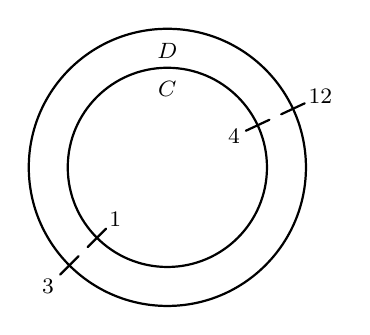
\begin{tikzpicture}[scale=1.1, line cap=round, line join=round]
    \draw[thick] (0, 0) circle (1.6cm);
    \draw[thick] (0, 0) circle (1.15cm);
    
    \node at (0, 1.35) {\footnotesize $D$};
    \node at (0, 0.9) {\footnotesize $C$};
    
    \draw[thick] (25:1.0) -- (25:1.3);
    \draw[thick] (25:1.45) -- (25:1.75);
    \node at (25:0.85) {\footnotesize $4$};
    \node at (25:1.95) {\footnotesize $12$};
    
    \draw[thick] (225:1.0) -- (225:1.3);
    \draw[thick] (225:1.45) -- (225:1.75);
    \node at (225:0.85) {\footnotesize $1$};
    \node at (225:1.95) {\footnotesize $3$};
\end{tikzpicture}
\end{center}

\subsection*{習題 5-7}
\begin{enumerate}
    \item 應用 D 尺及 K 尺求下列各數的立方：
    \begin{enumerate}[(i)]
        \item $2.14$,
        \item $5$,
        \item $2.72$,
        \item $3.66$.
    \end{enumerate}
    \item 應用 D 尺及 K 尺求下列各數的立方根：
    \begin{enumerate}[(i)]
        \item $10$,
        \item $100$,
        \item $343$,
        \item $493$.
    \end{enumerate}
    \item 欲求 $x, y$ 的幾何平均，請寫出用計算尺運算的程序.
    \item 自己試着造一根計算尺.
    \item 假設 $L, M, N$ 是三條對數尺度的直線，互相平行，且有相同距離，如下圖所示. 在 $L, N$ 兩線上各取點 $x, z$，連接 $xz$ 交 $M$ 線於 $y$ 點，求 $y$ 和 $x, z$ 的關係.
    
    \begin{center}
    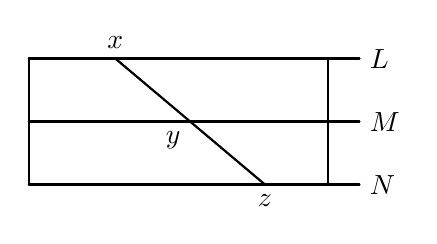
\begin{tikzpicture}[scale=1.0, line cap=round, line join=round]
        \draw[thick] (0, 0) rectangle (3.8, 1.6);
        \draw[thick] (0, 1.6) -- (4.2, 1.6) node[right] {$L$};
        \draw[thick] (0, 0.8) -- (4.2, 0.8) node[right] {$M$};
        \draw[thick] (0, 0) -- (4.2, 0) node[right] {$N$};
        
        \coordinate (X) at (1.1, 1.6);
        \coordinate (Y) at (2.05, 0.8);
        \coordinate (Z) at (3.0, 0);
        \draw[thick] (X) -- (Z);
        
        \node[above] at (X) {$x$};
        \node[below left] at (Y) {$y$};
        \node[below] at (Z) {$z$};
    \end{tikzpicture}
    \end{center}
    
    \item 如圖，兩平行線 $AC$ 及 $BD$ 交一角 $LOM$ 的兩邊於 $A, C, B, D$，若用 $x, y, u, v$, 各表示 $\overline{OA}, \overline{OB}, \overline{OC}, \overline{OD}$，則
    \[
    x : y = u : v, \text{ 卽 } xv = yu.
    \]
    想想看如何利用這個式子造出一個乘除用的計算器械！
    
    \begin{center}
    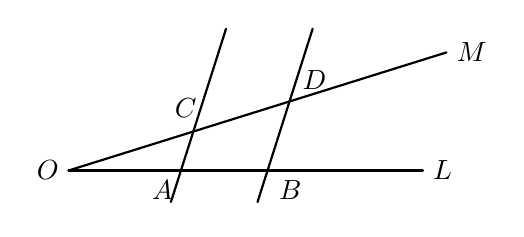
\begin{tikzpicture}[scale=1.0, line cap=round, line join=round]
        \coordinate (O) at (0, 0);
        \draw[thick] (O) -- (4.5, 0) node[right] {$L$};
        \draw[thick] (O) -- (4.8, 1.5) node[right] {$M$};
        \node[left] at (O) {$O$};
        
        \draw[thick] (1.3, -0.4) -- (2.0, 1.8);
        \draw[thick] (2.4, -0.4) -- (3.1, 1.8);
        
        \node[below left] at (1.45, 0) {$A$};
        \node[below right] at (2.55, 0) {$B$};
        \node[above left] at (1.75, 0.55) {$C$};
        \node[above right] at (2.85, 0.9) {$D$};
    \end{tikzpicture}
    \end{center}
\end{enumerate}

\clearpage
\subsection*{附錄：常用對數表}
\addcontentsline{toc}{subsection}{附錄：常用對數表}

\subsubsection*{對數表（1）}
{\centering\fontsize{7.5pt}{8.8pt}\selectfont\setlength{\tabcolsep}{1.5pt}\renewcommand{\arraystretch}{0.96}
\begin{tabular}{|c|cccccccccc|ccccccccc|}
\hline
數 & 0 & 1 & 2 & 3 & 4 & 5 & 6 & 7 & 8 & 9 & 1 & 2 & 3 & 4 & 5 & 6 & 7 & 8 & 9 \\ \hline
1.0 & .0000 & .0043 & .0086 & .0128 & .0170 & .0212 & .0253 & .0294 & .0334 & .0374 & 4 & 8 & 12 & 17 & 21 & 25 & 29 & 33 & 37 \\
1.1 & .0414 & .0453 & .0492 & .0531 & .0569 & .0607 & .0645 & .0682 & .0719 & .0755 & 4 & 8 & 11 & 15 & 19 & 23 & 26 & 30 & 34 \\
1.2 & .0792 & .0828 & .0864 & .0899 & .0934 & .0969 & .1004 & .1038 & .1072 & .1106 & 3 & 7 & 10 & 14 & 17 & 21 & 24 & 28 & 31 \\
1.3 & .1139 & .1173 & .1206 & .1239 & .1271 & .1303 & .1335 & .1367 & .1399 & .1430 & 3 & 6 & 10 & 13 & 16 & 19 & 23 & 26 & 29 \\
1.4 & .1461 & .1492 & .1523 & .1553 & .1584 & .1614 & .1644 & .1673 & .1703 & .1732 & 3 & 6 & 9 & 12 & 15 & 18 & 21 & 24 & 27 \\
1.5 & .1761 & .1790 & .1818 & .1847 & .1875 & .1903 & .1931 & .1959 & .1987 & .2014 & 3 & 6 & 8 & 11 & 14 & 17 & 20 & 22 & 25 \\
1.6 & .2041 & .2068 & .2095 & .2122 & .2148 & .2175 & .2201 & .2227 & .2253 & .2279 & 3 & 5 & 8 & 11 & 13 & 16 & 18 & 21 & 24 \\
1.7 & .2304 & .2330 & .2355 & .2380 & .2405 & .2430 & .2455 & .2480 & .2504 & .2529 & 2 & 5 & 7 & 10 & 12 & 15 & 17 & 20 & 22 \\
1.8 & .2553 & .2577 & .2601 & .2625 & .2648 & .2672 & .2695 & .2718 & .2742 & .2765 & 2 & 5 & 7 & 9 & 12 & 14 & 16 & 19 & 21 \\
1.9 & .2788 & .2810 & .2833 & .2856 & .2878 & .2900 & .2923 & .2945 & .2967 & .2989 & 2 & 4 & 7 & 9 & 11 & 13 & 16 & 18 & 20 \\
2.0 & .3010 & .3032 & .3054 & .3075 & .3096 & .3118 & .3139 & .3160 & .3181 & .3201 & 2 & 4 & 6 & 8 & 11 & 13 & 15 & 17 & 19 \\
2.1 & .3222 & .3243 & .3263 & .3284 & .3304 & .3324 & .3345 & .3365 & .3385 & .3404 & 2 & 4 & 6 & 8 & 10 & 12 & 14 & 16 & 18 \\
2.2 & .3424 & .3444 & .3464 & .3483 & .3502 & .3522 & .3541 & .3560 & .3579 & .3598 & 2 & 4 & 6 & 8 & 10 & 12 & 14 & 15 & 17 \\
2.3 & .3617 & .3636 & .3655 & .3674 & .3692 & .3711 & .3729 & .3747 & .3766 & .3784 & 2 & 4 & 6 & 7 & 9 & 11 & 13 & 15 & 17 \\
2.4 & .3802 & .3820 & .3838 & .3856 & .3874 & .3892 & .3909 & .3927 & .3945 & .3962 & 2 & 4 & 5 & 7 & 9 & 11 & 12 & 14 & 16 \\
2.5 & .3979 & .3997 & .4014 & .4031 & .4048 & .4065 & .4082 & .4099 & .4116 & .4133 & 2 & 3 & 5 & 7 & 9 & 10 & 12 & 14 & 15 \\
2.6 & .4150 & .4166 & .4183 & .4200 & .4216 & .4232 & .4249 & .4265 & .4281 & .4298 & 2 & 3 & 5 & 7 & 8 & 10 & 11 & 13 & 15 \\
2.7 & .4314 & .4330 & .4346 & .4362 & .4378 & .4393 & .4409 & .4425 & .4440 & .4456 & 2 & 3 & 5 & 6 & 8 & 9 & 11 & 13 & 14 \\
2.8 & .4472 & .4487 & .4502 & .4518 & .4533 & .4548 & .4564 & .4579 & .4594 & .4609 & 2 & 3 & 5 & 6 & 8 & 9 & 11 & 12 & 14 \\
2.9 & .4624 & .4639 & .4654 & .4669 & .4683 & .4698 & .4713 & .4728 & .4742 & .4757 & 1 & 3 & 4 & 6 & 7 & 9 & 10 & 12 & 13 \\
3.0 & .4771 & .4786 & .4800 & .4814 & .4829 & .4843 & .4857 & .4871 & .4886 & .4900 & 1 & 3 & 4 & 6 & 7 & 9 & 10 & 11 & 13 \\
3.1 & .4914 & .4928 & .4942 & .4955 & .4969 & .4983 & .4997 & .5011 & .5024 & .5038 & 1 & 3 & 4 & 6 & 7 & 8 & 10 & 11 & 12 \\
3.2 & .5051 & .5065 & .5079 & .5092 & .5105 & .5119 & .5132 & .5145 & .5159 & .5172 & 1 & 3 & 4 & 5 & 7 & 8 & 9 & 11 & 12 \\
3.3 & .5185 & .5198 & .5211 & .5224 & .5237 & .5250 & .5263 & .5276 & .5289 & .5302 & 1 & 3 & 4 & 5 & 6 & 8 & 9 & 10 & 12 \\
3.4 & .5315 & .5328 & .5340 & .5353 & .5366 & .5378 & .5391 & .5403 & .5416 & .5428 & 1 & 3 & 4 & 5 & 6 & 8 & 9 & 10 & 11 \\
3.5 & .5441 & .5453 & .5465 & .5478 & .5490 & .5502 & .5514 & .5527 & .5539 & .5551 & 1 & 2 & 4 & 5 & 6 & 7 & 9 & 10 & 11 \\
3.6 & .5563 & .5575 & .5587 & .5599 & .5611 & .5623 & .5635 & .5647 & .5658 & .5670 & 1 & 2 & 4 & 5 & 6 & 7 & 8 & 10 & 11 \\
3.7 & .5682 & .5694 & .5705 & .5717 & .5729 & .5740 & .5752 & .5763 & .5775 & .5786 & 1 & 2 & 3 & 5 & 6 & 7 & 8 & 9 & 10 \\
3.8 & .5798 & .5809 & .5821 & .5832 & .5843 & .5855 & .5866 & .5877 & .5888 & .5899 & 1 & 2 & 3 & 5 & 6 & 7 & 8 & 9 & 10 \\
3.9 & .5911 & .5922 & .5933 & .5944 & .5955 & .5966 & .5977 & .5988 & .5999 & .6010 & 1 & 2 & 3 & 4 & 5 & 7 & 8 & 9 & 10 \\
4.0 & .6021 & .6031 & .6042 & .6053 & .6064 & .6075 & .6085 & .6096 & .6107 & .6117 & 1 & 2 & 3 & 4 & 5 & 6 & 8 & 9 & 10 \\
4.1 & .6128 & .6138 & .6149 & .6160 & .6170 & .6180 & .6191 & .6201 & .6212 & .6222 & 1 & 2 & 3 & 4 & 5 & 6 & 7 & 8 & 9 \\
4.2 & .6232 & .6243 & .6253 & .6263 & .6274 & .6284 & .6294 & .6304 & .6314 & .6325 & 1 & 2 & 3 & 4 & 5 & 6 & 7 & 8 & 9 \\
4.3 & .6335 & .6345 & .6355 & .6365 & .6375 & .6385 & .6395 & .6405 & .6415 & .6425 & 1 & 2 & 3 & 4 & 5 & 6 & 7 & 8 & 9 \\
4.4 & .6435 & .6444 & .6454 & .6464 & .6474 & .6484 & .6493 & .6503 & .6513 & .6522 & 1 & 2 & 3 & 4 & 5 & 6 & 7 & 8 & 9 \\
4.5 & .6532 & .6542 & .6551 & .6561 & .6571 & .6580 & .6590 & .6599 & .6609 & .6618 & 1 & 2 & 3 & 4 & 5 & 6 & 7 & 8 & 9 \\
4.6 & .6628 & .6637 & .6646 & .6656 & .6665 & .6675 & .6684 & .6693 & .6702 & .6712 & 1 & 2 & 3 & 4 & 5 & 6 & 7 & 7 & 8 \\
4.7 & .6721 & .6730 & .6739 & .6749 & .6758 & .6767 & .6776 & .6785 & .6794 & .6803 & 1 & 2 & 3 & 4 & 5 & 5 & 6 & 7 & 8 \\
4.8 & .6812 & .6821 & .6830 & .6839 & .6848 & .6857 & .6866 & .6875 & .6884 & .6893 & 1 & 2 & 3 & 4 & 4 & 5 & 6 & 7 & 8 \\
4.9 & .6902 & .6911 & .6920 & .6928 & .6937 & .6946 & .6955 & .6964 & .6972 & .6981 & 1 & 2 & 3 & 4 & 4 & 5 & 6 & 7 & 8 \\
5.0 & .6990 & .6998 & .7007 & .7016 & .7024 & .7033 & .7042 & .7050 & .7059 & .7067 & 1 & 2 & 3 & 3 & 4 & 5 & 6 & 7 & 8 \\
5.1 & .7076 & .7084 & .7093 & .7101 & .7110 & .7118 & .7126 & .7135 & .7143 & .7152 & 1 & 2 & 3 & 3 & 4 & 5 & 6 & 7 & 8 \\
5.2 & .7160 & .7168 & .7177 & .7185 & .7193 & .7202 & .7210 & .7218 & .7226 & .7235 & 1 & 2 & 2 & 3 & 4 & 5 & 6 & 7 & 7 \\
5.3 & .7243 & .7251 & .7259 & .7267 & .7275 & .7284 & .7292 & .7300 & .7308 & .7316 & 1 & 2 & 2 & 3 & 4 & 5 & 6 & 6 & 7 \\
5.4 & .7324 & .7332 & .7340 & .7348 & .7356 & .7364 & .7372 & .7380 & .7388 & .7396 & 1 & 2 & 2 & 3 & 4 & 5 & 6 & 6 & 7 \\
\hline
\end{tabular}\par}

\vspace{0.5em}
\noindent $\log \pi = 0.4971$

\clearpage
\subsubsection*{對數表（2）}
{\centering\fontsize{7.5pt}{8.8pt}\selectfont\setlength{\tabcolsep}{1.5pt}\renewcommand{\arraystretch}{0.96}
\begin{tabular}{|c|cccccccccc|ccccccccc|}
\hline
數 & 0 & 1 & 2 & 3 & 4 & 5 & 6 & 7 & 8 & 9 & 1 & 2 & 3 & 4 & 5 & 6 & 7 & 8 & 9 \\ \hline
5.5 & .7404 & .7412 & .7419 & .7427 & .7435 & .7443 & .7451 & .7459 & .7466 & .7474 & 1 & 2 & 2 & 3 & 4 & 5 & 5 & 6 & 7 \\
5.6 & .7482 & .7490 & .7497 & .7505 & .7513 & .7520 & .7528 & .7536 & .7543 & .7551 & 1 & 2 & 2 & 3 & 4 & 5 & 5 & 6 & 7 \\
5.7 & .7559 & .7566 & .7574 & .7582 & .7589 & .7597 & .7604 & .7612 & .7619 & .7627 & 1 & 2 & 2 & 3 & 4 & 5 & 5 & 6 & 7 \\
5.8 & .7634 & .7642 & .7649 & .7657 & .7664 & .7672 & .7679 & .7686 & .7694 & .7701 & 1 & 1 & 2 & 3 & 4 & 4 & 5 & 6 & 7 \\
5.9 & .7709 & .7716 & .7723 & .7731 & .7738 & .7745 & .7752 & .7760 & .7767 & .7774 & 1 & 1 & 2 & 3 & 4 & 4 & 5 & 6 & 7 \\
6.0 & .7782 & .7789 & .7796 & .7803 & .7810 & .7818 & .7825 & .7832 & .7839 & .7846 & 1 & 1 & 2 & 3 & 4 & 4 & 5 & 6 & 6 \\
6.1 & .7853 & .7860 & .7868 & .7875 & .7882 & .7889 & .7896 & .7903 & .7910 & .7917 & 1 & 1 & 2 & 3 & 4 & 4 & 5 & 6 & 6 \\
6.2 & .7924 & .7931 & .7938 & .7945 & .7952 & .7959 & .7966 & .7973 & .7980 & .7987 & 1 & 1 & 2 & 3 & 3 & 4 & 5 & 6 & 6 \\
6.3 & .7993 & .8000 & .8007 & .8014 & .8021 & .8028 & .8035 & .8041 & .8048 & .8055 & 1 & 1 & 2 & 3 & 3 & 4 & 5 & 5 & 6 \\
6.4 & .8062 & .8069 & .8075 & .8082 & .8089 & .8096 & .8102 & .8109 & .8116 & .8122 & 1 & 1 & 2 & 3 & 3 & 4 & 5 & 5 & 6 \\
6.5 & .8129 & .8136 & .8142 & .8149 & .8156 & .8162 & .8169 & .8176 & .8182 & .8189 & 1 & 1 & 2 & 3 & 3 & 4 & 5 & 5 & 6 \\
6.6 & .8195 & .8202 & .8209 & .8215 & .8222 & .8228 & .8235 & .8241 & .8248 & .8254 & 1 & 1 & 2 & 3 & 3 & 4 & 5 & 5 & 6 \\
6.7 & .8261 & .8267 & .8274 & .8280 & .8287 & .8293 & .8299 & .8306 & .8312 & .8319 & 1 & 1 & 2 & 3 & 3 & 4 & 5 & 5 & 6 \\
6.8 & .8325 & .8331 & .8338 & .8344 & .8351 & .8357 & .8363 & .8370 & .8376 & .8382 & 1 & 1 & 2 & 3 & 3 & 4 & 4 & 5 & 6 \\
6.9 & .8388 & .8395 & .8401 & .8407 & .8414 & .8420 & .8426 & .8432 & .8439 & .8445 & 1 & 1 & 2 & 2 & 3 & 4 & 4 & 5 & 6 \\
7.0 & .8451 & .8457 & .8463 & .8470 & .8476 & .8482 & .8488 & .8494 & .8500 & .8506 & 1 & 1 & 2 & 2 & 3 & 4 & 4 & 5 & 6 \\
7.1 & .8513 & .8519 & .8525 & .8531 & .8537 & .8543 & .8549 & .8555 & .8561 & .8567 & 1 & 1 & 2 & 2 & 3 & 4 & 4 & 5 & 5 \\
7.2 & .8573 & .8579 & .8585 & .8591 & .8597 & .8603 & .8609 & .8615 & .8621 & .8627 & 1 & 1 & 2 & 2 & 3 & 4 & 4 & 5 & 5 \\
7.3 & .8633 & .8639 & .8645 & .8651 & .8657 & .8663 & .8669 & .8675 & .8681 & .8686 & 1 & 1 & 2 & 2 & 3 & 4 & 4 & 5 & 5 \\
7.4 & .8692 & .8698 & .8704 & .8710 & .8716 & .8722 & .8727 & .8733 & .8739 & .8745 & 1 & 1 & 2 & 2 & 3 & 3 & 4 & 5 & 5 \\
7.5 & .8751 & .8756 & .8762 & .8768 & .8774 & .8779 & .8785 & .8791 & .8797 & .8802 & 1 & 1 & 2 & 2 & 3 & 3 & 4 & 5 & 5 \\
7.6 & .8808 & .8814 & .8820 & .8825 & .8831 & .8837 & .8842 & .8848 & .8854 & .8859 & 1 & 1 & 2 & 2 & 3 & 3 & 4 & 5 & 5 \\
7.7 & .8865 & .8871 & .8876 & .8882 & .8887 & .8893 & .8899 & .8904 & .8910 & .8915 & 1 & 1 & 2 & 2 & 3 & 3 & 4 & 4 & 5 \\
7.8 & .8921 & .8927 & .8932 & .8938 & .8943 & .8949 & .8954 & .8960 & .8965 & .8971 & 1 & 1 & 2 & 2 & 3 & 3 & 4 & 4 & 5 \\
7.9 & .8976 & .8982 & .8987 & .8993 & .8998 & .9004 & .9009 & .9015 & .9020 & .9025 & 1 & 1 & 2 & 2 & 3 & 3 & 4 & 4 & 5 \\
8.0 & .9031 & .9036 & .9042 & .9047 & .9053 & .9058 & .9063 & .9069 & .9074 & .9079 & 1 & 1 & 2 & 2 & 3 & 3 & 4 & 4 & 5 \\
8.1 & .9085 & .9090 & .9096 & .9101 & .9106 & .9112 & .9117 & .9122 & .9128 & .9133 & 1 & 1 & 2 & 2 & 3 & 3 & 4 & 4 & 5 \\
8.2 & .9138 & .9143 & .9149 & .9154 & .9159 & .9165 & .9170 & .9175 & .9180 & .9186 & 1 & 1 & 2 & 2 & 3 & 3 & 4 & 4 & 5 \\
8.3 & .9191 & .9196 & .9201 & .9206 & .9212 & .9217 & .9222 & .9227 & .9232 & .9238 & 1 & 1 & 2 & 2 & 3 & 3 & 4 & 4 & 5 \\
8.4 & .9243 & .9248 & .9253 & .9258 & .9263 & .9269 & .9274 & .9279 & .9284 & .9289 & 1 & 1 & 2 & 2 & 3 & 3 & 4 & 4 & 5 \\
8.5 & .9294 & .9299 & .9304 & .9309 & .9315 & .9320 & .9325 & .9330 & .9335 & .9340 & 1 & 1 & 2 & 2 & 3 & 3 & 4 & 4 & 5 \\
8.6 & .9345 & .9350 & .9355 & .9360 & .9365 & .9370 & .9375 & .9380 & .9385 & .9390 & 1 & 1 & 2 & 2 & 3 & 3 & 4 & 4 & 5 \\
8.7 & .9395 & .9400 & .9405 & .9410 & .9415 & .9420 & .9425 & .9430 & .9435 & .9440 & 0 & 1 & 1 & 2 & 2 & 3 & 3 & 4 & 4 \\
8.8 & .9445 & .9450 & .9455 & .9460 & .9465 & .9469 & .9474 & .9479 & .9484 & .9489 & 0 & 1 & 1 & 2 & 2 & 3 & 3 & 4 & 4 \\
8.9 & .9494 & .9499 & .9504 & .9509 & .9513 & .9518 & .9523 & .9528 & .9533 & .9538 & 0 & 1 & 1 & 2 & 2 & 3 & 3 & 4 & 4 \\
9.0 & .9542 & .9547 & .9552 & .9557 & .9562 & .9566 & .9571 & .9576 & .9581 & .9586 & 0 & 1 & 1 & 2 & 2 & 3 & 3 & 4 & 4 \\
9.1 & .9590 & .9595 & .9600 & .9605 & .9609 & .9614 & .9619 & .9624 & .9628 & .9633 & 0 & 1 & 1 & 2 & 2 & 3 & 3 & 4 & 4 \\
9.2 & .9638 & .9643 & .9647 & .9652 & .9657 & .9661 & .9666 & .9671 & .9675 & .9680 & 0 & 1 & 1 & 2 & 2 & 3 & 3 & 4 & 4 \\
9.3 & .9685 & .9689 & .9694 & .9699 & .9703 & .9708 & .9713 & .9717 & .9722 & .9727 & 0 & 1 & 1 & 2 & 2 & 3 & 3 & 4 & 4 \\
9.4 & .9731 & .9736 & .9741 & .9745 & .9750 & .9754 & .9759 & .9763 & .9768 & .9773 & 0 & 1 & 1 & 2 & 2 & 3 & 3 & 4 & 4 \\
9.5 & .9777 & .9782 & .9786 & .9791 & .9795 & .9800 & .9805 & .9809 & .9814 & .9818 & 0 & 1 & 1 & 2 & 2 & 3 & 3 & 4 & 4 \\
9.6 & .9823 & .9827 & .9832 & .9836 & .9841 & .9845 & .9850 & .9854 & .9859 & .9863 & 0 & 1 & 1 & 2 & 2 & 3 & 3 & 4 & 4 \\
9.7 & .9868 & .9872 & .9877 & .9881 & .9886 & .9890 & .9894 & .9899 & .9903 & .9908 & 0 & 1 & 1 & 2 & 2 & 3 & 3 & 4 & 4 \\
9.8 & .9912 & .9917 & .9921 & .9926 & .9930 & .9934 & .9939 & .9943 & .9948 & .9952 & 0 & 1 & 1 & 2 & 2 & 3 & 3 & 4 & 4 \\
9.9 & .9956 & .9961 & .9965 & .9969 & .9974 & .9978 & .9983 & .9987 & .9991 & .9996 & 0 & 1 & 1 & 2 & 2 & 3 & 3 & 3 & 4 \\
\hline
\end{tabular}\par}
